\documentclass[tikz,border=8pt]{standalone}
\usepackage{amsmath}
\usetikzlibrary{arrows.meta,calc}
\definecolor{ink}{HTML}{21352F}\definecolor{teal}{HTML}{087F7B}
\definecolor{blue}{HTML}{4B77A8}\definecolor{gold}{HTML}{C58B2A}
\begin{document}
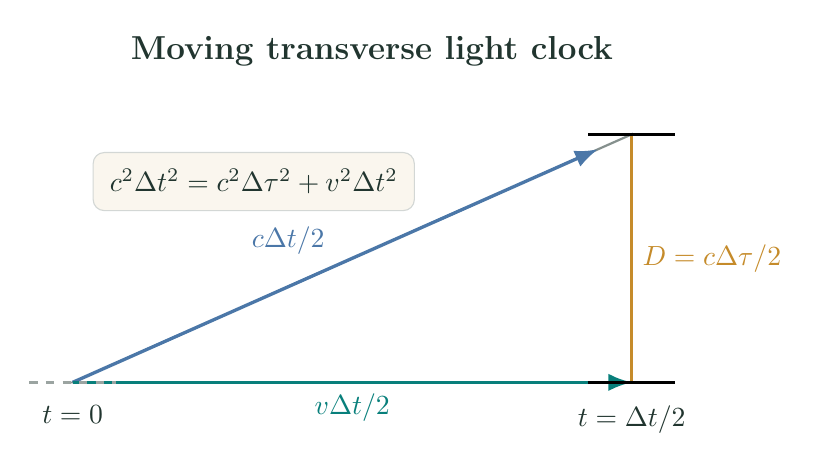
\begin{tikzpicture}[font=\sffamily,text=ink,>=Latex]
  \node[font=\bfseries\large] at (0,4.2) {Moving transverse light clock};
  \coordinate (A) at (-3.8,0); \coordinate (B) at (3.3,0); \coordinate (C) at (3.3,3.15);
  \draw[ink!55,thick] (A)--(B)--(C)--cycle;
  \draw[blue,very thick,->] (A)--($(A)!.94!(C)$) node[midway,above left] {$c\Delta t/2$};
  \draw[teal,very thick,->] (A)--(B) node[midway,below] {$v\Delta t/2$};
  \draw[gold,very thick] (B)--(C) node[midway,right] {$D=c\Delta\tau/2$};
  \draw[very thick,ink!45,dashed] ($(A)+(-.55,0)$)--($(A)+(.55,0)$);
  \draw[very thick] ($(B)+(-.55,0)$)--($(B)+(.55,0)$);
  \draw[very thick] ($(C)+(-.55,0)$)--($(C)+(.55,0)$);
  \node[below=5pt] at (A) {$t=0$};
  \node[below=5pt] at (B) {$t=\Delta t/2$};
  \node[draw=ink!20,fill=gold!8,rounded corners=4pt,inner sep=6pt] at (-1.5,2.55)
    {$c^2\Delta t^2=c^2\Delta\tau^2+v^2\Delta t^2$};
\end{tikzpicture}
\end{document}
